\documentclass[11pt]{article}
\usepackage[T1]{fontenc}
\usepackage{lmodern}
\usepackage{parskip}
\usepackage[colorlinks=true,urlcolor=Blue,linkcolor=black,citecolor=black]{hyperref}
\usepackage{graphicx}
\usepackage{amsmath}
\usepackage[utf8]{inputenc}
\usepackage[spanish]{babel}
\usepackage{fancyhdr}
\usepackage{csquotes}
\usepackage{lastpage}
\usepackage{array}
\usepackage{listings}
\usepackage{color}
\definecolor{dkgreen}{rgb}{0,0.6,0}
\definecolor{gray}{rgb}{0.5,0.5,0.5}
\definecolor{mauve}{rgb}{0.58,0,0.82}
\usepackage[affil-it]{authblk}
\usepackage[activate={true,nocompatibility},final,tracking=true,kerning=true,spacing=true,factor=1100,stretch=10,shrink=10]{microtype}
\usepackage[hmargin=2cm,top=4cm,headheight=65pt,footskip=65pt]{geometry}

% Graphicx Path
\graphicspath{ {./images/} }

% Para el código de Turtle
\lstset{frame=tb,
  language=Turtle,
  aboveskip=3mm,
  belowskip=3mm,
  showstringspaces=false,
  columns=flexible,
  basicstyle={\small\ttfamily},
  numbers=none,
  numberstyle=\tiny\color{gray},
  keywordstyle=\color{blue},
  commentstyle=\color{dkgreen},
  stringstyle=\color{mauve},
  breaklines=true,
  breakatwhitespace=true,
  tabsize=3
}

% Documento
\begin{document}
% Título
\title{SIW PL9. Extracción de información semántica.}
\author{Hugo Fonseca Díaz\\ \email{uo258318@uniovi.es}}
\affil{Escuela de Ingeniería Informática. Universidad de Oviedo.}
\maketitle
% Ejercicio 1
\section{Información estructurada}
En esta primera sección se obtendrá información estructurada de tres textos mediante el uso de tipos definidos en \verb|schema.org| \cite{schemaorg}. Dicha información se define a continuación:

\begin{itemize}
    \item \textbf{Miles Davis:} es una entidad de tipo \verb|Person|. Sus propiedades son:
        \begin{itemize}
            \item \verb|familyName|: Davis
            \item \verb|givenName|: Miles
            \item \verb|hasOccupation|: \verb|Occupation|(\verb|name|: jazz musician)
            \item \verb|nationality|: \verb|Country|(\verb|name|: United States of America)
            \item \verb|url|: \url{https://www.wikidata.org/wiki/Q93341}
        \end{itemize}
    \item \textbf{Barack Obama:} es una entidad de tipo \verb|Person|. Sus propiedades son:
        \begin{itemize}
            \item \verb|familyName|: Obama
            \item \verb|givenName|: Barack
            \item \verb|hasOccupation|: \verb|Occupation|(\verb|name|: President)
            \item \verb|url|: \url{https://www.wikidata.org/wiki/Q76}
        \end{itemize}
    \item \textbf{European Union:} es una entidad de tipo \verb|Organization|. Sus propiedades son:
        \begin{itemize}
            \item \verb|name|: European Union
            \item \verb|legalName|: European Union
            \item \verb|url|: \url{https://www.wikidata.org/wiki/Q458}
        \end{itemize}
    \item \textbf{Washington:} es una entidad de tipo \verb|City|. Sus propiedades son:
        \begin{itemize}
            \item \verb|name|: Washington DC
            \item \verb|url|: \url{https://www.wikidata.org/wiki/Q61}
        \end{itemize}
    \item \textbf{Euro a Dólar:} es una entidad de tipo \verb|ExchangeRateSpecification|. Sus propiedades son:
        \begin{itemize}
            \item \verb|currency|: EUR
            \item \verb|currentExchangeRate|: \verb|UnitPriceSpecification|(\verb|priceCurrency|: USD, \verb|price|: 1.3)
            \item \verb|url|: \url{https://www.ecb.europa.eu/stats/policy_and_exchange_rates/euro_reference_exchange_rates/html/index.en.html}
        \end{itemize}
    \item \textbf{The New York Times:} es una entidad de tipo \verb|Newspaper|. Sus propiedades son:
        \begin{itemize}
            \item \verb|name|: The New York Times
            \item \verb|url|: \url{https://www.wikidata.org/wiki/Q9684}
        \end{itemize}
    \item \textbf{John McCarthy:} es una entidad de tipo \verb|Person|. Sus propiedades son:
        \begin{itemize}
            \item \verb|familyName|: McCarthy
            \item \verb|givenName|: John
            \item \verb|hasOccupation|: \verb|Occupation|(\verb|name|: computer scientist)
            \item \verb|url|: \url{https://www.wikidata.org/wiki/Q92739}
        \end{itemize}
    \item \textbf{LISP:} es una entidad de tipo \verb|ComputerLanguage|. Sus propiedades son:
        \begin{itemize}
            \item \verb|name|: LISP
            \item \verb|url|: \url{https://www.wikidata.org/wiki/Q132874}
        \end{itemize}
\end{itemize}
\section{Modelado RDF}
En esta sección se muestra el modelado \textit{RDF} en formato \textit{Turtle} con el que se ha representado la información listada previamente. Dicho modelado es el siguiente:

\begin{lstlisting}
@prefix schema: <https://schema.org/> .
@prefix wikidata: <https://wikidata.org/> .
@prefix rdf:<http://www.w3.org/1999/02/22-rdf-syntax-ns#> .

# Primer texto
wikidata:Q93341 rdf:type schema:Person ;
    schema:familyName "Davis" ;
    schema:givenName "Miles" ;
    schema:hasOccupation [
        rdf:type schema:Occupation ;
        schema:name "jazz musician"
    ] ;
    schema:nationality wikidata:Q30 .

# Segundo texto
wikidata:Q76 rdf:type schema:Person ;
    schema:familyName "Obama" ;
    schema:givenName "Barack" ;
    schema:hasOccupation [
        rdf:type schema:Occupation ;
        schema:name "president"
    ] .

wikidata:Q458 rdf:type schema:Organization ;
    schema:name "European Union" ;
    schema:legalName "European Union" .

wikidata:Q61 rdf:type schema:City ;
    schema:name "Washington DC" .

<https://www.ecb.europa.eu/stats/policy_and_exchange_rates/euro_reference_exchange_rates/html/index.en.html> rdf:type schema:ExchangeRateSpecification ;
    schema:currency "EUR" ;
    schema:currentExchangeRate [
        rdf:type schema:UnitPriceSpecification ;
        schema:priceCurrency "USD" ;
        schema:price 1.3
    ] .

# Tercer texto
wikidata:Q9684 rdf:type schema:Newspaper ;
    schema:name "The New York Times" .

wikidata:Q92739 rdf:type schema:Person ;
    schema:familyName "McCarthy" ;
    schema:givenName "John" ;
    schema:hasOccupation [
        rdf:type schema:Occupation ;
        schema:name "computer scientist"
    ] .

wikidata:Q132874 rdf:type schema:ComputerLanguage ;
    schema:name "LISP" .
\end{lstlisting}

En la \textbf{Figura 1} se observa el output de la herramienta \textit{RDFShape} al introducir el fichero en formato \textit{Turtle}. Se observa que el fichero está bien formado. Una vez hecho eso, convertimos el fichero a \textit{JSON-LD} mediante el uso de la herramienta \textit{RDF Translator} \cite{rdftranslator}. En la \textbf{Figura 2} se puede ver la validación de la \textit{Google Structured Data Testing Tool} \cite{googlesdtt} sobre el \textit{JSON-LD} generado previamente.

\begin{figure}[h]
\caption{Validación del fichero \textit{Turtle} mediante la herramienta \textit{RDFShape}.}
\centering
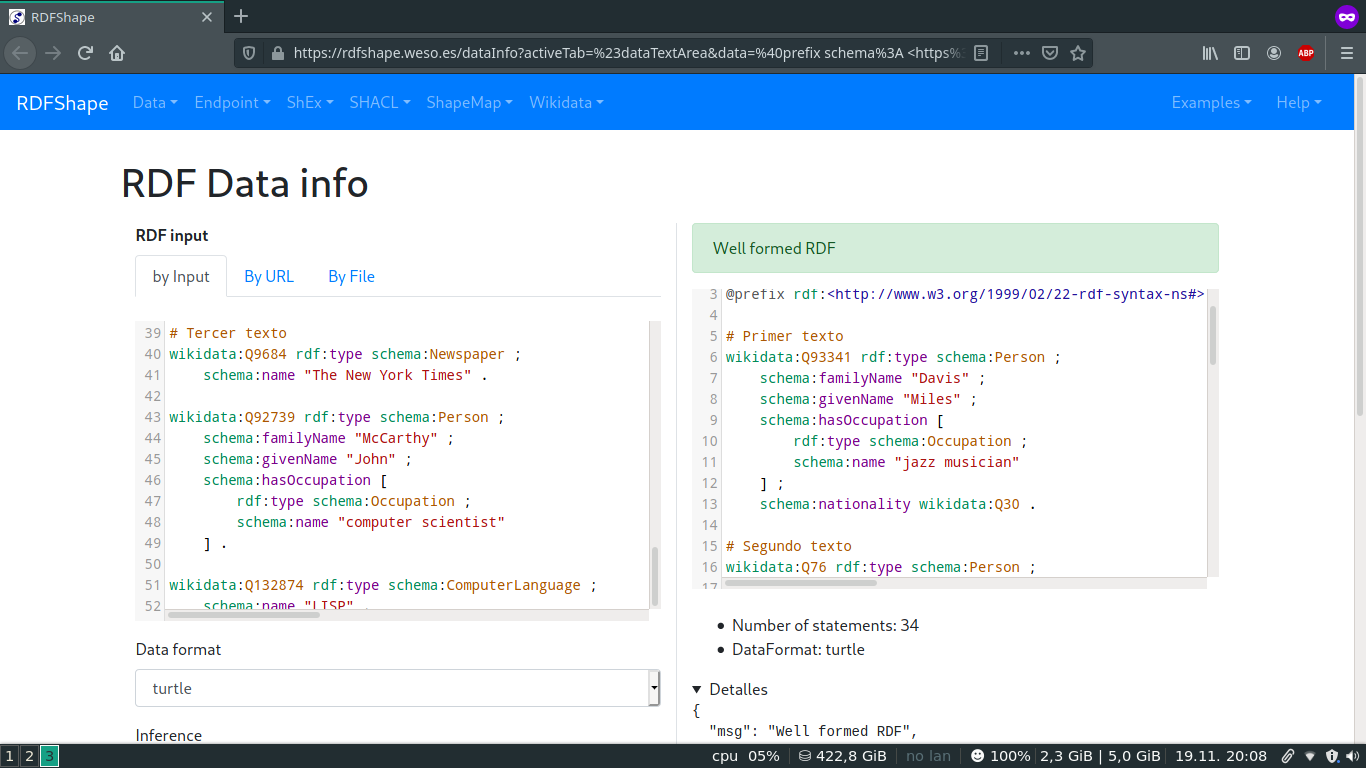
\includegraphics[width=\textwidth]{weso_turtle}
\end{figure}

\begin{figure}[h]
\caption{Validación del fichero \textit{JSON-LD} mediante la herramienta \textit{Google Structured Data Testing Tool}.}
\centering
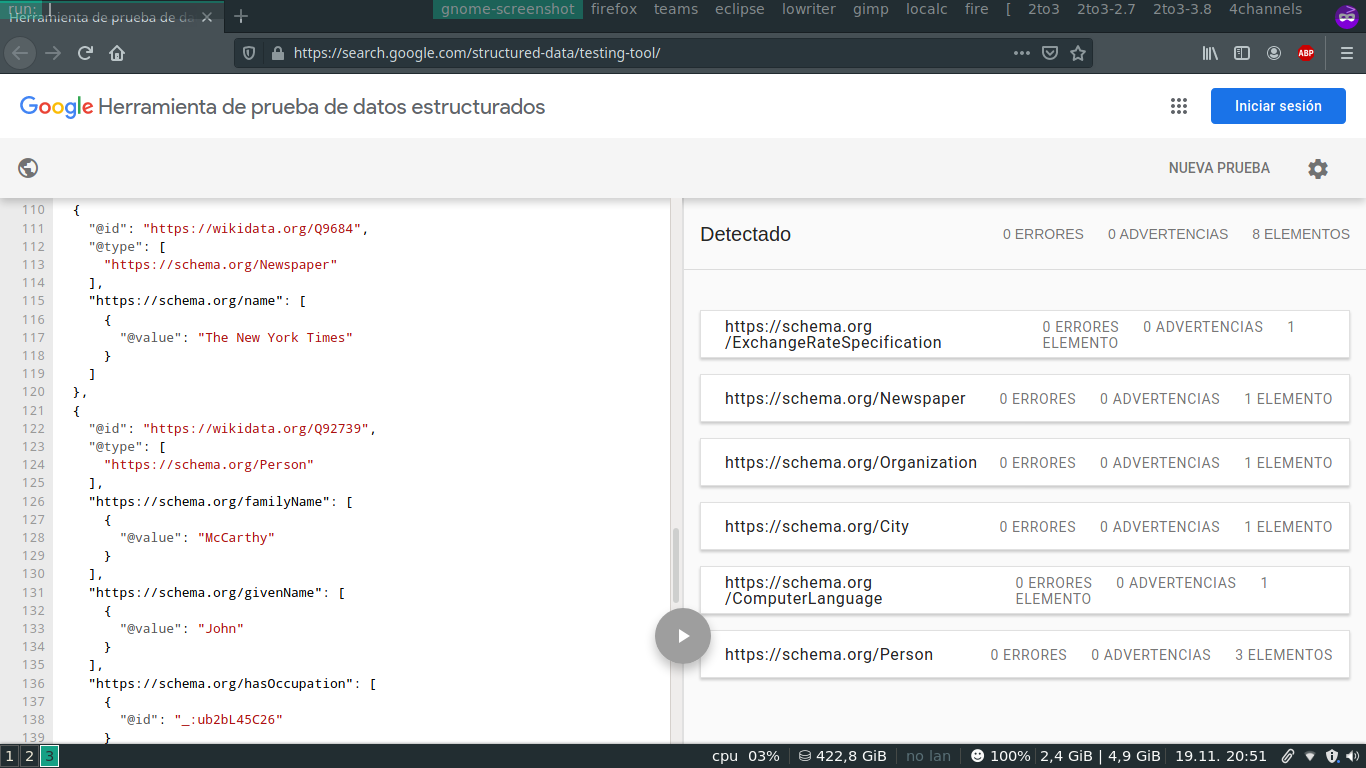
\includegraphics[width=\textwidth]{google_jsonld}
\end{figure}
\section{Obtención automática de información estructurada}
En esta parte del documento se procederá a obtener información estructurada mediante el uso de varias herramientas. Estas son \textit{Intelligent Tagging} de \textit{PermID} \cite{permid}, \textit{DBpedia Spotlight} \cite{dbpedia} y \textit{FRED} \cite{fred}.

A continuación se muestra una serie de ejemplos en forma de capturas de pantalla. Estos ejemplos ilustrarían el proceso realizado para obtener la información estructurada por medio de la herramienta \textit{FRED} para el texto \textit{“Miles Davis was an american jazz musician.”}. En la \textbf{Figura 3} se muestra la herramienta \textit{FRED} con el texto en lenguaje natural. En la \textbf{Figura 4} se muestra la conversión a \textit{JSON-LD} del fichero \textit{RDF-XML} obtenido en el previo paso (también se transforma a \textit{N3} para una inspección manual, aunque no se muestra en la captura). Por último, en la \textbf{Figura 5} se muestra la validación del fichero \textit{JSON-LD}. Estos pasos se realizan para todos los textos y los ficheros obtenidos pueden observarse en las carpetas adjuntadas a este documento.

\begin{figure}[h]
\caption{Obtención del fichero en formato \textit{RDF-XML} mediante la herramienta \textit{FRED}.}
\centering
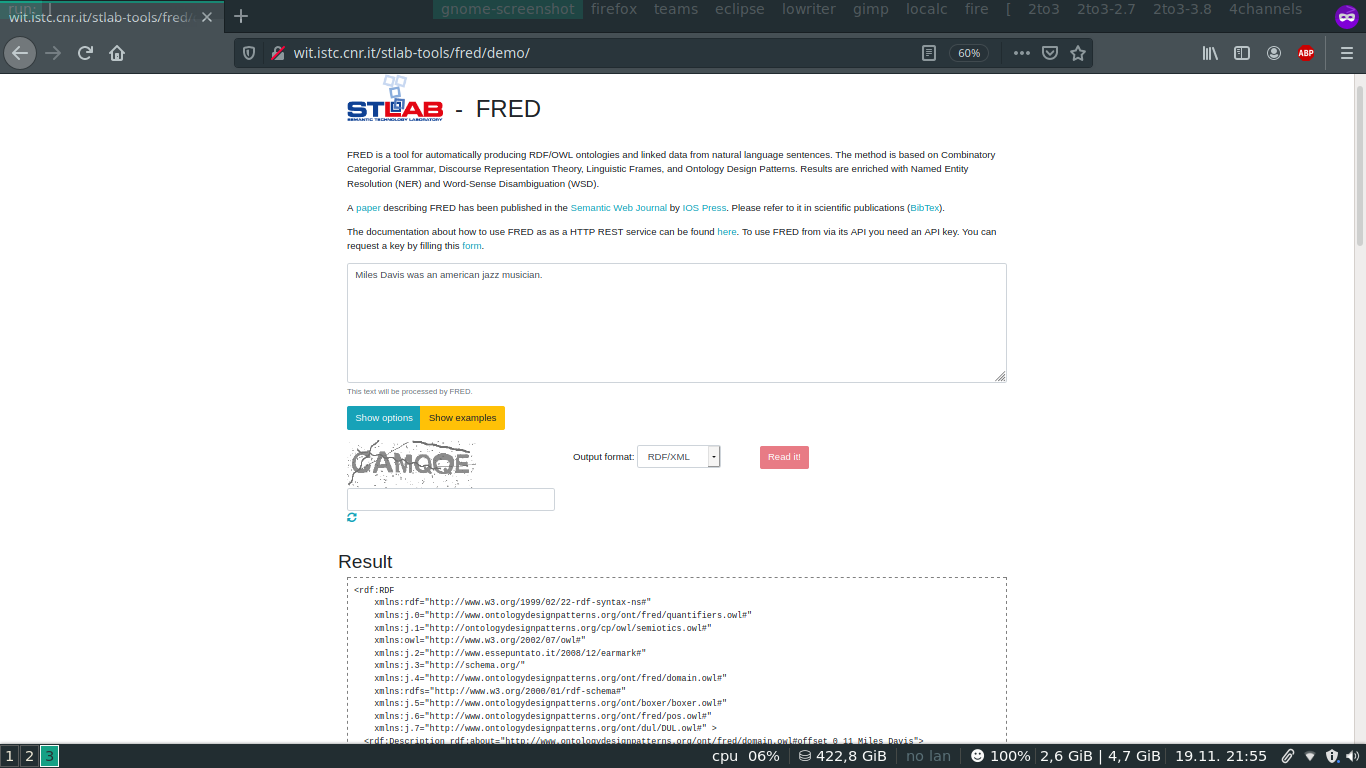
\includegraphics[width=\textwidth]{fred_1}
\end{figure}

\begin{figure}[h]
\caption{Obtención del fichero en formato \textit{JSON-LD} mediante la herramienta \textit{RDF Translator}.}
\centering
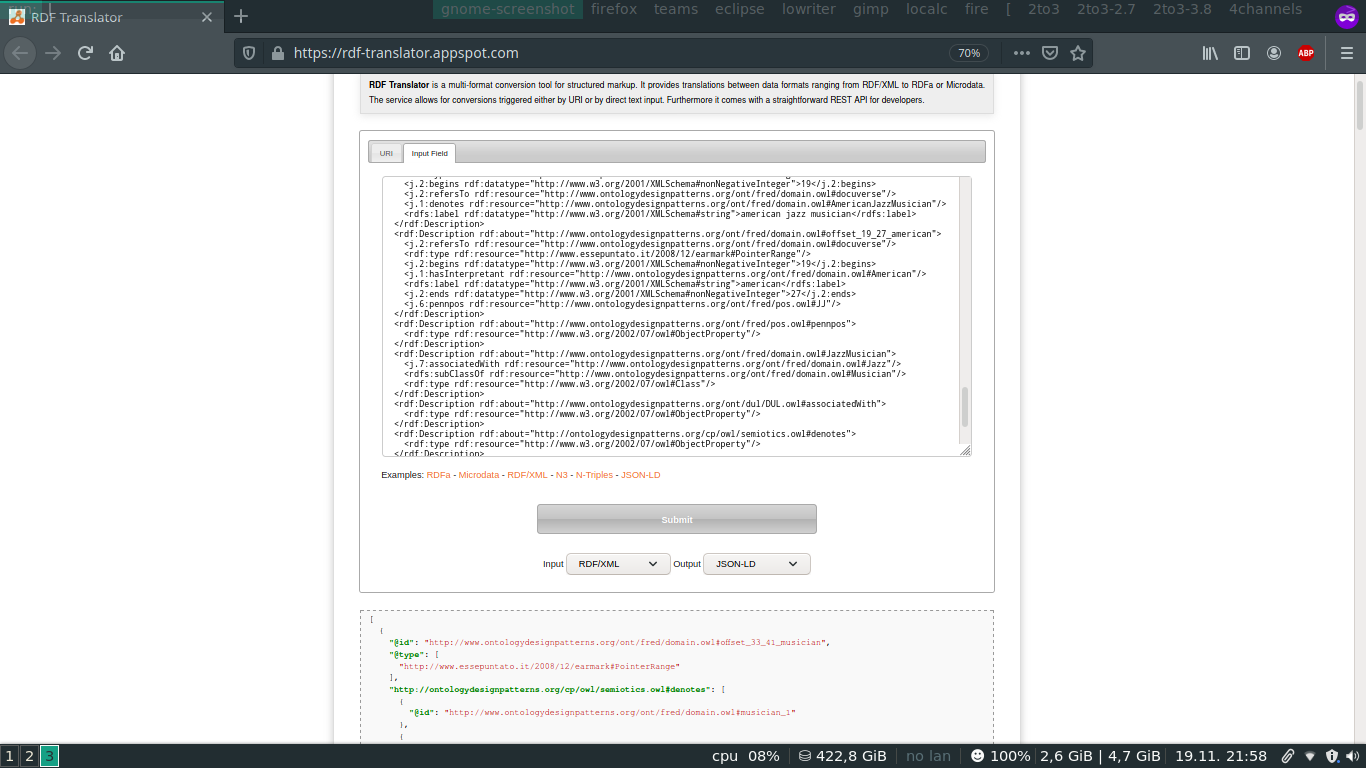
\includegraphics[width=\textwidth]{fred_2}
\end{figure}

\begin{figure}[h]
\caption{Validación del fichero \textit{JSON-LD} mediante la herramienta \textit{Google Structured Data Testing Tool}.}
\centering
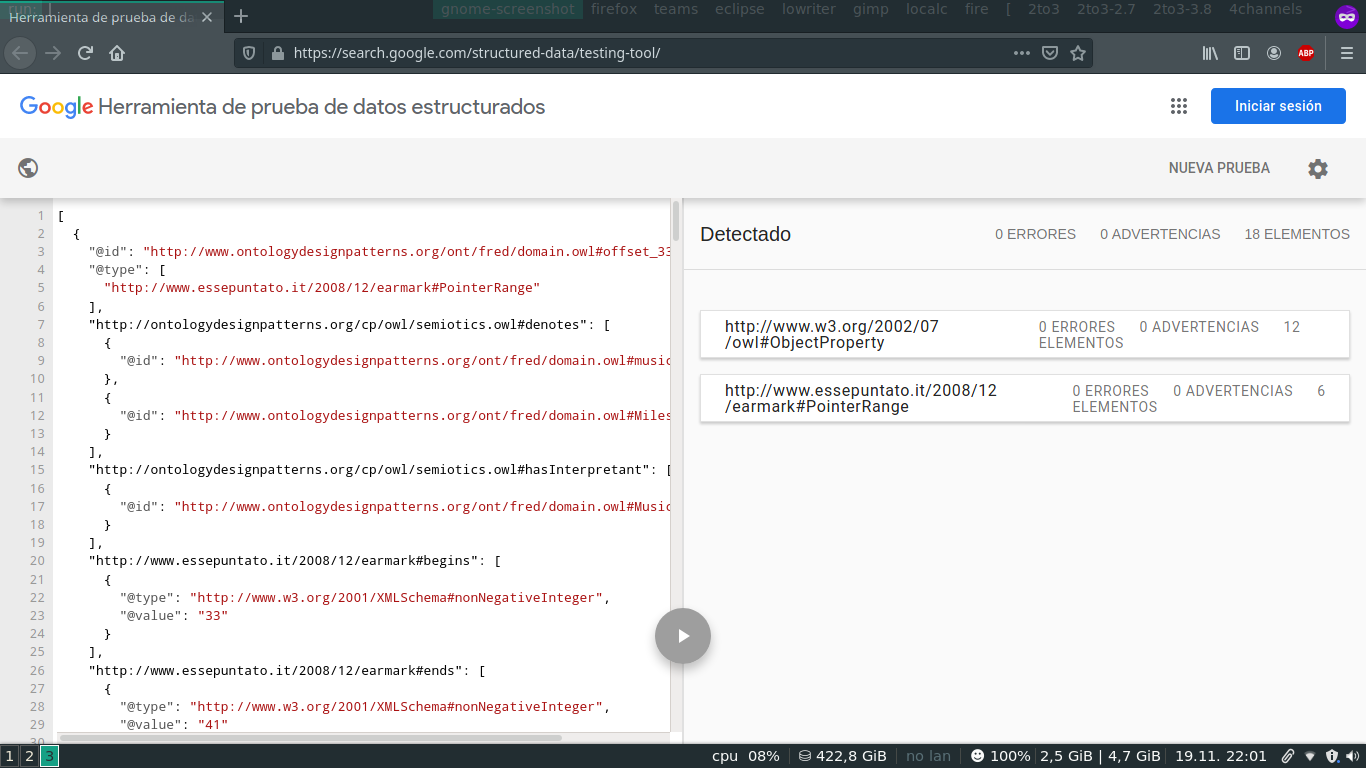
\includegraphics[width=\textwidth]{fred_3}
\end{figure}
% Bibliografía
\begin{thebibliography}{8}
\bibitem{schemaorg}
Página de \textit{Schema.org}, \url{https://schema.org/}. Última vez accedido 19 de noviembre de 2020.        

\bibitem{rdftranslator}
Página del \textit{RDF Translator}, \url{https://rdf-translator.appspot.com/}. Última vez accedido 19 de noviembre de 2020.

\bibitem{googlesdtt}
Página de la \textit{Google Structured Data Testing Tool}, \url{https://search.google.com/structured-data/testing-tool/}. Última vez accedido 19 de noviembre de 2020.

\bibitem{permid}
Página de la herramienta \textit{Intelligent Tagging} de \textit{Refinitiv}, \url{https://permid.org/onecalaisViewer}. Última vez accedido 19 de noviembre de 2020.

\bibitem{dbpedia}
Página de la herramienta \textit{DBpedia Spotlight}, \url{https://www.dbpedia-spotlight.org/demo/}. Última vez accedido 19 de noviembre de 2020.

\bibitem{fred}
Página de la herramienta \textit{FRED}, \url{http://wit.istc.cnr.it/stlab-tools/fred/demo/}. Última vez accedido 19 de noviembre de 2020.
\end{thebibliography}
\end{document}
